\section{Introduction}

In recent years, Large Language Models (LLMs)~\citep{team2023gemini, yang2025qwen3, liu2024deepseek, dubey2024llama,anthropic2025claude4, openai2025gpt5} have developed rapidly, demonstrating powerful capabilities across multiple domains. However, significant challenges remain when deploying these models as the core of AI agents designed to handle real-world tasks.
While existing agents have achieved remarkable progress on standardized benchmarks such as question answering~\citep{rein2024gpqa}, mathematical reasoning~\citep{lu2023mathvista, aime}, and code generation~\citep{chen2021codex}, these evaluations are limited to measuring domain-specific abilities.
To assess the general-purpose capabilities, researchers design benchmarks in interactive environments such as OSWorld~\citep{xie2024osworld} and WebArena~\citep{zhou2023webarena}. Yet, these environments still fall short, typically evaluating isolated functionalities within a single platform through short-horizon tasks of roughly 20 steps.
In contrast, real-world \textit{Productivity Tasks} represent a higher order of complexity. 
These tasks are characterized by long-horizon planning and interaction—potentially exceeding a hundred steps—and require agents to fluidly switch across multiple diverse applications.
Such complexity demands advanced agent capabilities in long-term planning, robust interaction,  and seamless cross-application tool integration.



\begin{wrapfigure}[24]{!t}{0.5\textwidth} 
    \centering
    \vspace{-10pt}
    % \includegraphics[width=\linewidth]{./figs/QA_teaser_demo.png}
    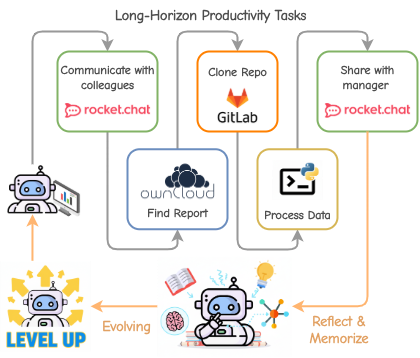
\includegraphics[width=\linewidth]{./figures/teaser.png}
    \caption{Illustration of the test-time learning and evolution of {\method} agents on long-horison, productivity tasks. The agent explores and accumulates experience in a cross-application interactive environment, constantly enriching its memory, thereby achieving continuous improvement.}
    \label{fig:teaser}
\end{wrapfigure}


Furthermore, most existing agents are \textit{test-time static}: their capabilities are fixed once the LLM training phase ends. As a result, each time an agent tackles a task, it operates like an amnesiac executor, unable to effectively learn from past experiences and lacking the capacity for continuous learning and self-evolution. Neither successes nor failures from previous tasks can be consolidated into effective knowledge to guide future actions. Consequently, even if an agent has successfully completed a task before, there is no guarantee of stable replication. When faced with repetitive tasks, it cannot improve efficiency through practice as humans do. This ``one-off'' interaction model severely limits agent performance in complex and dynamic environments, making test-time learning difficult to implement and revealing a core deficit in the ability to truly \textit{learn on the job}.


To address persistent challenges in dynamic planning, experience accumulation, and continuous learning for existing agents, we propose a novel agent framework \textbf{\method}, which stands for \textbf{M}emory-\textbf{U}tilizing and \textbf{S}elf-\textbf{E}volving. As illustrated in Figure~\ref{fig:teaser}, the core of {\method} is an experience-driven, closed-loop system centered around a Memory Module. This module hierarchically organizes diverse levels of knowledge, including procedural knowledge, strategic patterns, and tool-use guidance. Operating within a cross-application interactive environment, the agent leverages its accumulated experience to plan and explore solutions for long-horizon productivity tasks. After each sub-task, the agent reflects on its execution trajectory and distills reusable experience back into the Memory Module.
By converting raw action sequences into structured knowledge, {\method} enhances the applicability of experience and reduces redundant exploration. 
This mechanism effectively extends the agent's competence beyond its static pretrained parameters, fostering a dynamically evolving system with superior robustness and adaptability. Crucially, since the memory is stored in natural language, the accumulated knowledge is LLM-agnostic, allowing experience gained by one model to be seamlessly transferred and utilized by another.


We evaluate our framework on TheAgentCompany (TAC)~\citep{xu2024theagentcompanybenchmarkingllmagents}, a benchmark designed for long-horizon productivity tasks. Our experiments demonstrate that as the agent autonomously continuously accumulates experience within the working environment, it exhibits increasingly superior task completion capabilities and its capacity for continuous learning and self-evolution. Furthermore, our {\method} achieves new SOTA performance by a significant margin, using only a lightweight Gemini-2.5 Flash model. Our contributions are threefold:

\begin{itemize}

    \item We present the {\method} framework, featuring an experience-driven closed-loop architecture. It empowers agents to dynamically accumulate experiences through interaction with working environments, enabling them to evolve beyond LLM's static pretrained parameters.
    
    \item {\method} autonomously converts raw action trajectories into structured, reusable memory without human intervention, aiming to reduce redundant exploration and steadily improve agent performance. Its natural language format enables seamless knowledge transfer across different LLMs.

    \item We establish a new SOTA on the long-horizon productivity task benchmark TAC with a score of 51.78\%, achieving a 20\% relative leap over the previous SOTA. Extended experiments demonstrate the effectiveness of our framework's continuous learning and self-evolution capabilities.
    
\end{itemize}



